\documentclass[a4paper,10pt]{book}

\usepackage[brazil]{babel}    % dá suporte para os termos na língua portuguesa do Brasil
\usepackage[T1]{fontenc}      % Lê a codificação de fonte T1 (font encoding default é 0T1).
\usepackage{lmodern}        % Fonte "Latin Modern", experimente no lugar de ae
\usepackage{times}
\usepackage{t1enc}         % Fonte "Times New", experimente no lugar de ae
%\usepackage[latin1]{inputenc}
\usepackage[utf8]{inputenc} % acentuação em UTF8 (comente as linhas de inputenc, fontenc e ae)
                              % Caso tenha problemas ao usar UTF-8, experimente \usepackage{ucs}
\usepackage{indentfirst}       % indenta os primeiros parágrafos
\usepackage{amssymb,amsmath}   % simbolos matemáticos providos pela AMS
\usepackage[dvipdfm]{graphicx} % para inclusão de figuras (png, jpg, gif, bmp)
\usepackage{graphics}          % figuras gráficas
\usepackage{color}             % para letras e caixas coloridas
\usepackage{makeidx}           % índice remissivo
\usepackage{a4wide}            % correta formatação da página em A4
\usepackage{setspace}          % para a distância entre linhas
\usepackage{html}
\usepackage{ulem}
\usepackage{longtable} %para tabelas longas
\usepackage{array}
\usepackage[table]{xcolor}
\usepackage{wrapfig}
\usepackage[pdftex]{hyperref}
\usepackage{longtable}

%\usepackage{minitoc}

\newcommand\ead{\hbox{EAD}}
\newcommand\ufpb{\hbox{UFPB}}
\newcommand\ava{\hbox{AVA}}
\newcommand\moodle{\hbox{Moodle}}
\newcommand\uab{\hbox{UAB}}

\newcommand\atencao[1]{\textbf{}}


\newcommand{\red}[1]{\textcolor{red}{#1} }
\newcommand{\blue}[1]{\textcolor{blue}{#1} }


\makeindex

\title{Conte com Moodle no Próximo Semestre \\ \mbox{} \\ \includegraphics[width=2.0cm]{imagem/cap0/hat.jpg}}
\author{UFPB Virtual}
\date{April - 2013}

\begin{document}

\maketitle

\pagenumbering{roman}

\cleardoublepage
\begin{center}
\quad

\vspace*{0.9\textheight}

 \parbox[t]{0.7\textwidth}{Texto produzido para uso dos tutores e professores da UFPB Virtual.}
\parbox[t]{12cm}{Registrado sob licença Creative Commons (\url{www.creativecommons.org})}
\end{center}

\index{Ubuntu}
\index{Kile}
\index{Creative Commons}
\index{Moodle 1.9.3$^+$}

\tableofcontents
%\listoffigures

\mainmatter
\chapter{Introdução}

%\minitoc
Desde os primórdios da história da humanidade, o ambiente de ensino tem tido um papel
importante na difusão do conhecimento. Antigamente, o conhecimento era passado
verbalmente de uma geração para outra. Com o desenvolvimento de técnicas de
impressão, o conhecimento
passou a ser armazenado em livros possibilitando assim a disseminação maior do conhecimento. 
Finalmente com a democratização da educação, o conhecimento passou a ser disseminado em massa 
através de aulas \emph{presenciais}, onde professores ensinam na presença física dos seus alunos. 

Com o advento e popularização dos computadores e da Internet 
estamos vivendo uma nova transição em como disseminar conhecimento na forma da \emph{Educação à Distância} (\ead). 
No \ead, alunos participam de aulas virtuais transmitidas pela Internet
diretamente nos seus computadores
e professores podem acompanhar os seus alunos à distância através de atividades como 
fóruns de discussão, pesquisas de opinião, e atividades também transmitidas
pela Internet.

Na última década, o \ead\ tem se popularizado e ganhado dimensões comparáveis ao do ensino  
tradicional. Universidades de renome internacional, como a Universidade de Stanford e o \emph{Massachusetts Institute of 
Technology} (MIT) nos Estados Unidos, tem aberto cursos universitários online. Também no contexto brasileiro, 
universidades, como a Universidade de São Paulo (USP), já oferecem cursos 
à distância que tem a mesma validade e prestígio que os seus curso presenciais. 
A Universidade Federal da Paraíba (\ufpb), por exemplo, abriu cursos de licenciatura em 
diversas áreas, como Administração Pública, Ciências Agrárias, Ciências Biológicas, Ciências Naturais,
Computação, Letras, Letras/Libras, Matemática e Pedagogia. O objetivo destes cursos
é de atender as necessidades de ensino das regiões da Paraíba e do Nordeste sem acesso fácil
à educação superior de qualidade. 

O sucesso destes cursos pode ser evidenciado pelo número de inscritos nesses vestibulares e pela taxa de 
evasão. Os números abaixo são do curso à distância de licenciatura em letras da Universidade Federal da Paraíba, fornecidos pela 
coordenação do curso:
\begin{itemize}
 \item De 2007 até 2013 foram oferecidas 3180 vagas das quais 3126 foram preenchidas. 
 Quer dizer uma média de um pouco mais de 220 vagas por semestre;
 
 \item A taxa de evasão \red{durante este período} foi de de cerca de 
35 por cento, equiparável, se não melhor que, no ensino presencial.
\end{itemize}
 Os outros cursos à distância oferecidos pela \ufpb\  tem números similares.

\index{Estatísticas do \ead} 
 
\red{ Estes números sugerem que existe demanda clara para o ensino à distância e que os alunos escritos
terminam o curso apesar de ser um curso de ensino à distância.  Contudo, outra questão é sobre a 
qualidade dos cursos à distância. 
O resultado obtido Exame Nacional de Desempenho de Estudantes (Enade). }

Grande parte deste sucesso se deve ao bom uso dos Ambientes Virtuais de Aprendizagem (\ava) disponíveis para
o Ensino à Distância. Ao contrário do ensino presencial, onde os educadores tem contato direto 
com os seus alunos em períodos bem estabelecidos na forma de aulas presenciais, 
no Ensino à Distância os educadores interagem com os seus alunos na maior parte do tempo 
através do Ambiente Virtual de Aprendizagem. $\ava$s são aplicativos que rodam em um servidor 
conectado na Internet rodando 24 horas por dia 7 dias por semana. Educadores montam a sua disciplina em um \ava, o qual é acessado 
por seus alunos através dos seus computadores com acesso a Internet usando navegadores como Firefox, Chrome ou Internet Explorer. 
Num \ava\ um educador pode por exemplo:
\begin{itemize}
 \item inserir o seu material didático como apresentações, textos, ou mesmo links para outras páginas ou vídeos;
 \item publicar atividades como tarefas de casa e provas;
 \item iniciar uma discussão de um tema específico através de um fórum, onde alunos postam comentários a 
 respeito do tema;
 \item consultar os seus alunos através de pesquisas de opinião para determinar
formas de melhorar a sua metodologia de ensino como também entender melhor as
maiores dificuldades dos seus alunos;
 \item inserir os métodos de avaliação e calcular as notas dos alunos;
 \item examinar relatórios gerandos usando os dados de acesso dos seus alunos que são 
coletados pelo AVA.
\end{itemize}
Este leque de ferramentas disponíveis em $\ava$s abre caminhos para criar técnicas de ensino 
mais criativas e mais eficazes que as técnicas normalmente usados no ensino presencial
baseadas somente no uso do quadro e de slides. As ferramentas em um \ava\ permite  
o educador monitorar de maneira mais sistemática o avanço e deficiências dos seus alunos, 
levando o aluno a aumentar o interesse pela disciplina, mesmo que o ensino não seja presencial. 

Entretanto, devido ao número grande de ferramentas disponíveis, muitos educadores que não tem experiência 
com AVAs se sentem perdidos e não conseguem usar estas ferramentas de maneira efetiva. 
Este manual tem portanto a finalidade de ajudar educadores a como usarem o Ambiente Virtual de Aprendizado
chamado \emph{\moodle}. O \moodle\ é um dos $\ava$s de maior sucesso sendo utilizado por diversas 
universidade ao redor do mundo. As informações neste manual foram frutos de um 
estudo de práticas de sucesso que observamos no uso do \moodle\ 
nos cursos de ensino à distância da Universidade Federal da Paraíba. 

No resto deste capítulo iremos na Seção~\ref{subsec:cap1:Ead} dar uma visão geral de como uma disciplina
é ministrada em um curso de Educação à Distância e na Seção~\ref{subsec:cap1:Moodle} iremos motivar o
uso do \moodle.

\section{Como Funciona a Educação à Distância (UAB)}
\label{subsec:cap1:Ead}

Existem diversas modalidades de Educação à Distância. \red{quais?} 

O Ministério da Educação do Governo brasileiro elaborou no ano de 2005 o modelo de 
\emph{Universidade Aberta do Brasil} (\uab) adotadas nos cursos à distância das 
universidades brasileiras. O objetivo deste modelo é de atender as necessidades 
das comunidades sem acesso fácil a educação superior oferecendo cursos superiores de qualidade.
Nesta seção iremos abordar o modelo \uab\ de educação que é usado nos cursos à distância oferecidos pela
Universidade Federal da Paraíba.

Na \uab, as instituições de ensino colaboram com os governos municipais e 
estaduais. Enquanto as instituições de ensino fornecem o material didático e capacitação 
dos educadores, os governos municipais e estaduais fornecem a infra-estrutura básica 
para os seus alunos na forma de Pólos. Nos pólos encontram-se as laboratórios onde
os alunos dos cursos podem acessar as disciplinas. Durante o semestre, professores
da instituições de ensino visitam por um breve período os pólos para ter um contato mais direto com os 
seus alunos. 
\begin{figure}[htbp]
 \begin{center}
 \fbox{\includegraphics[width=0.35\textwidth]{imagem/cap1/fig1.jpg}}
  \caption{Cenário ilustrando as relações entre os Pólos e as Instituições de Ensino}
  \label{fig:UAB}
 \end{center}
\end{figure}

A Figura~\ref{fig:UAB}, obtida do site da UAB\footnote{\url{http://www.uab.capes.gov.br/}}, 
ilustra bem o funcionamento desta colaboração. Neste cenário, existem três instituições
de ensino e três pólos. As instituições de ensino oferecem alguns cursos para os seus 
pólos. Por exemplo, a instituição de ensino 1 (IES1) oferece o curso A ao Pólo 1 e 
o curso B ao pólo 2. Como ilustra a figura, diferentes instituições de ensino podem
compartilhar a infra-estrutura dos pólos para oferecer cursos complementares aos pólos.

Como um curso presencial, os cursos à distância tem uma grade curricular formado 
por um conjunto de disciplinas. Para o aluno se formar, este precisa passar as disciplinas
exigidas pelo curso. Numa disciplina de um curso à distância existem três tipos de educadores:
\begin{itemize}
 \item \textbf{Professores} -- Os professores são educadores que já tem experiência no ensino do tópico 
 abordado pela disciplina, tendo a ensinado em cursos presenciais ou à distância. Ele é o responsável 
 pela disciplina. Além de ter as funções usuais de um professor em uma disciplina presencial, como 
 elaborar provas, 
 o professor em uma disciplina à distância deve planejar a disciplina, acompanhar os tutores, e montar a sala de aula 
 no Ambiente Virtual de Aprendizado. O professor deve, por exemplo, criar
atividades como fóruns, pesquisas de opinião ou dever de casa.
 Em alguns cursos também é exigido que o professor visite os pólos para ter um contato mais pessoal 
 com os seus alunos e tutores, assim melhorando a interação entre esses. 
 
 \item \textbf{Tutores à Distância} -- Os tutores à distância, normalmente situados nas instituições de ensino, 
 auxiliam os professores no ensino da disciplina. Eles são responsáveis por tirar dúvidas dos alunos e ajudá-los 
 nos exercícios. Como os tutores tem um contato maior com os alunos, percebendo quais são as maiores 
 dificuldades dos alunos da disciplina, é função dos tutores de comunicar aos professores as suas observações para
 que o professor possa melhor planejar os próximos passos da disciplina. 
 
 
 \item \textbf{Tutores Presenciais} -- Finalmente, os tutores presenciais são educadores que estão situados nos pólos
 propocionando a relação presencial necessária para um bom aprendizado. 
Além de controlar a frequência dos alunos, os tutores  ajudam os alunos que tem
dificuldades em acessar a sala do curso no 
 \ava, aplicam as provas elaboradas pelos professores nos pólos e 
 ajudam os alunos a usarem os recursos disponíveis nos $\ava$s. \red{O que mais?}
\end{itemize}

\red{Incluir uma tabela resumindo as responsabilidades dos tutores, professores e alunos}

\section{Diferenças ao Ensino Presencial}  Existem muitas diferenças entre o ensino presencial e 
o ensino à distância. Enquanto o contato no ensino presencial entre os educadores e os seus alunos acontece de maneira síncrona, 
quer dizer, em horários bem definidos, no ensino à distância, o contato entre os educadores e os seus alunos é de maneira
assíncrona, quer dizer, pode ocorrer em qualquer momento. Essa diferença faz com que muitas vezes as estratégias de ensino usadas no ensino 
presencial, como o uso de quadro e de slides, não sejam as mais adequadas no ensino à distância. O uso de outras ferramentas, 
como fóruns e bate-papos, se torna mais importante. Outra diferença é que o \ead\ exige uma coordenação maior entre os professores, tutores
à distância e tutores presenciais. Como o professor não tem contato físico com os alunos, ele precisa da avaliação dos tutores, 
que tem um contato diário com os alunos, para modelar a sua disciplina e escolher que tipo de atividade que deve ser usada.

De fato, \avas\ são desenvolvidos com o intuito de incentivar 
a \emph{interatividade} entre alunos, tutores e professores. Esta interatividade é formentada por ferramentas 
disponíveis nos \avas\ como fóruns, salas de bate-papo, formação de grupos, realização de atividades, entre outras. 
Enquanto na aulas presenciais muitos alunos hesitam em participar devido a diversos fatores como timidez, insegurança ou 
mesmo limitações de linguagem, muitos alunos tendem a ser mais abertos a discussões em 
fóruns virtuais como evidenciado nas redes sociais como Facebook e Twitter. 

Contudo assim como nas redes sociais, a discussão num ambiente virtual pode perder o foco e não atingir 
o seu objetivo final. Portanto tanto para professores como para tutores, é importante dominar os 
tipos de ferramentas disponíveis em um \ava\ para que professores e tutores possam transmitir 
de maneira efetiva o conhecimento da disciplina aos seus alunos.


\section{Ambientes Virtuais de Aprendizado: Moodle}
\label{subsec:cap1:Moodle}

Os Ambientes Virtuais de Aprendizado (\avas) são plataformas computacionais que rodam ininterruptamente em servidores 
conectados à Internet. O objetivo de uma \ava\ é de fornecer os recursos necessários para professores, tutores 
e alunos poderem collaborar a fim de permitir a Educação de Qualidade à Distância. Um \ava\ permite ao 
professor organizar sua disciplina na forma
de uma página da Internet. Esta página pode ser acessada por seus alunos e seus tutores que podem não somente ver o 
material postado pelo professor, mas também pode participar de atividades e interagir entre si através, de 
por exemplo, salas de bate-papo. Um \ava\ favorece portanto a criação de uma \emph{comunidade virtual} cujo objetivo 
é o aprendizado e disseminação do conhecimento.\footnote{No Apêndice~\ref{sec:apendice}, 
descrevemos como alunos dos cursos à distância da \ufpb\ pode acessar o site do Moodle do instituto.}

Um requisito básico para o uso de um \ava\ é o conhecimento básico de navegação Web. É esperado que um usuário 
saiba acessar uma página na Internet. 

Por que usar um AVA, por que usar o Moodle?

% \section{Ambiente Virtuais de Aprendizagem}
% 
% Desde o início dos anos 90 professores ouvem comentários sobre a revolução que vem sendo provocada pela Internet no ensino e na aprendizagem, mas essa revolução ainda não se materializou. Em lugar disso, um novo conjunto de ferramentas, chamado LMS (Learning Management System em inglês, Sistema de Gestão de Aprendizagem em português), ou AVA como é mais conhecido (Ambiente Virtual de Aprendizagem), pode ser usado para melhorar seus cursos, tirando proveito das vantagens da Internet sem dispensar a necessidade do professor. Nos últimos dez anos, os AVAs experimentaram um crescimento e amadurecimento rápidos e são, hoje, considerados essenciais em muitas universidades e faculdades.
% 
% 
% 
% \section{Ambientes Virtuais de Aprendizagem}
% 
% AVAs são aplicações Intra/Internet que “rodam” em um servidor web\footnote{Servidor web é um computador que está ligado 7 dias na semana, 24 horas por dia, à Internet, onde estão gravados os arquivos do Ava e onde está um banco de dados que guarda as informações das disciplinas e usuários, podendo ser acessadas mediante autenticação, pelos interessados em qualquer lugar onde haja conexão com a rede mundial de computadores.}  e são acessadas por um navegador (Internet Explorer, Monzila Firefox, Google Chrome, Ópera, Safari, etc.). O servidor está, no caso geral, localizado em um departamento ou centro de processamento de uma Universidade, mas pode estar localizado em qualquer lugar do mundo. O professor e os alunos podem acessar o sistema de qualquer lugar onde haja um computador, conexão com a Internet e um navegador Web. Em termos simples, um AVA fornece ao professor ferramentas para que ele crie um curso baseado em uma ambiente Web (site), com controle de acesso de forma tal que somente os alunos do curso 
% possam acessar o mesmo. Além deste controle, os AVAs oferecem uma variedade de ferramentas que podem aumentar a eficácia de um curso. Pode-se, facilmente, compartilhar materiais de estudo, manter discussões síncronas e assíncronas\footnote{Síncrona: que acontece em tempo real, ao mesmo tempo para todos os participantes. Assíncrona: que não está vinculada ao tempo, ou seja, a discussão pode ocorrer em períodos de tempo distintos, quando uma participação que ocorre agora é respondida depois e assim por diante.}, aplicar testes de avaliação e pesquisas de opinião, coletar e revisar tarefas, além de registrar notas. 
% 
% \index{síncrono}
% \index{assíncrono}
% 
% \section{Recursos AVA}
% \index{Recursos}
% Os ambientes AVAs provêem os mais variados recursos educacionais, no intuito de prover maior didática e eficiência na comunicação entre alunos e professores.  Podemos analisar alguns destes recursos a seguir.
% 
% \subsection{Enviando e compartilhando materiais de estudo}
% \index{Materiais de estudo}
% A maioria dos AVAs fornece ferramentas para publicar com facilidade, textos e outros materiais de estudo. Ao invés de usar um editor HTML\footnote{Hypertext Markup Language: Linguagem de Marcação para Hipertextos, usada para dar formatação às páginas web e criar vínculos (links) entre elas.} , e então, enviar o texto para um servidor Web, usa-se um formulário para publicar conteúdos (enviar arquivos). Muitos professores costumam publicar em um site da Internet todo o material que produzem e que pode ser útil para os seus alunos. Porém estes ambientes não possuem tantos recursos didáticos como o ambiente AVA.
% 
% 
% \subsection{Fóruns e Salas de bate-papo}
% 
% \index{Fóruns e chat}
% 
% Esses recursos fornecem meios de comunicação entre o professor e os alunos fora da sala de aula. Os fóruns proporcionam mais tempo para reflexão antes que a participação aconteça e permitem manter uma discussão por um período longo de tempo. As salas de bate-papo, por outro lado, fornecem uma forma de comunicação rápida e instantânea com professores, tutores e alunos. Podem ser usados para uma discussão aberta, com tema livre, ou até mesmo para uma aula virtual. Sabe-se de um professor que, impedido de falar por motivos médicos, conduz seu curso usando salas de bate-papo para se comunicar com os alunos. Outro uso comum é aquele feito por grupos de alunos que devem produzir um trabalho e usam o bate-papo online para se organizar e discutir detalhes do trabalho.
% 
% \subsection{Testes e pesquisas de opinião}
% 
% \index{Testes e pesquisas}
% 
% Testes online e pesquisas de opinião podem ser corrigidos e processados instantaneamente. São grandes ferramentas para 
% permitir que os alunos tenham uma informação rápida e eficaz auto-avaliação sobre seu desempenho no curso. É comum hoje em dia que editoras e autores de livros texto coloquem questionários sobre os capítulos de seus livros em sítios na Internet. Podermos citar um exemplo de um professor que conduzindo um curso sobre propaganda na Universidade de São Francisco (EUA), produz um banco de questões e adota mini-testes para verificar o progresso dos alunos em seus estudos. A prova final é um teste com questões retiradas de todo o banco, de maneira aleatória.
% 
% \subsection{Coletando e revisando tarefas}
% 
% \index{Revisão de tarefas}
% 
% Coletar, corrigir e revisar tarefas (divulgando os resultados da correção com comentários) é um trabalho cansativo e maçante. Tarefas online é uma forma fácil de coletar e corrigir trabalhos dos alunos e atribuir e divulgar notas. Além disso, pesquisas indicam que o uso de ambientes online com participação anônima, para que os alunos atribuam notas a trabalhos feitos por seus colegas, aumenta a motivação e o desempenho.
% 
% \subsection{Registrando notas}
% 
% \index{Registro de notas}
% 
% Um quadro de notas online permite que os alunos tenham informações sempre atualizadas sobre seu desempenho em um curso. Notas online também facilitam cumprir a determinação de algumas instituições de ensino de que não tornem públicas as avaliações dos alunos. Os quadros de notas dos AVAs permitem, em geral, que os alunos consultem apenas as próprias notas. É possível, ainda, copiar o quadro de notas para o computador do professor para processamentos mais elaborados. Embora seja possível encontrar (ou desenvolver) programas que façam este trabalho, um AVA tem essas ferramentas integradas em seu ambiente. 
% 
% \section{Por que usar um AVA?}
% 
% Aulas têm sido ministradas por milhares de anos sem o uso de computadores ou da Internet. O ambiente em que o professor utiliza um quadro negro, giz e conversa ainda são ferramentas dominantes no processo educacional. Embora o formato tradicional, ou seja, de forma presencial, possa ainda ser eficaz, o uso das ferramentas acima listadas abrem novas possibilidades de aprendizagem que não eram imagináveis há anos atrás.
% 
% No momento, uma grande quantidade de pesquisa ainda é feita sobre como combinar aprendizagem presencial com os chamados cursos híbridos. Que são os cursos que combinam aulas presenciais e aula à distância. Imagine transferir a maior parte do material didático de seu curso para um ambiente virtual e aproveitar seu tempo em aula para discussões, questões e resolução de problemas. Muitos professores já descobriram que eles podem economizar tempo e melhorar a aprendizagem de seus alunos comportando-se dessa maneira. Isto permite que os alunos usem os encontros presencias para a solução de problemas e os professores possam transformar suas aulas em palestras de contextualização, abandonando a preocupação de ter que cumprir o programa de forma presencial.
% 
% As discussões online permitem que muitos alunos se expressem em formas que eles não conseguiriam em aulas regulares. Muitos deles relutam em falar em aula por motivos variados: timidez, insegurança, ou mesmo limitações de linguagem. A possibilidade de criar um ambiente de construção coletiva do conhecimento online é, muitas vezes, de grande importância para alguns alunos. Muitos professores relatam um aumento significativo na participação quando se introduz esse formato de aprendizagem. Há outro número de razões para se pensar na utilização de ambientes virtuais em seus cursos, como por exemplo:
% 
% \begin{itemize}
%  \item Demanda dos alunos: os alunos (especialmente os de curso superior) têm, hoje, um grau de inclusão digital muito maior, e utilizam muitos sistemas de comunicação como (MSN, Facebook, GTalk, Skype, por exemplo) eles se sentem à vontade em um AVA;
%  \item Horários dos alunos: aumenta cada vez mais o número de alunos que trabalha. Em alguns países, a média semanal de trabalho dos alunos de cursos superiores chega a 20 horas. Com ambientes online eles podem adequar seus horários de trabalho às atividades de um curso;
%  \item Cursos melhores: se bem usado, um AVA pode tornar suas aulas mais eficazes e melhores. Movendo parte de seu curso para a Internet é possível aproveitar os encontros presenciais para envolver os alunos em questões básicas do curso e convidá-lo a refletir sobre temas correlatos. O professor pode, também, aproveitar o tempo discorrendo sobre temas que sempre desejou abordar e foi impedido pelo fato de ter que cumprir o programa.
% \end{itemize}
% 
% Você provavelmente ouviu os argumentos até aqui apresentados durante a última década do século XX. Então, o que mudou? Hoje, os AVAs estão melhores estruturados, mais maduros, e fáceis de usar do que foram há alguns anos atrás. A tecnologia que envolve a disponibilidade deste ambiente tornou-se melhor e mais estável. Há pouco tempo, muitos sistemas eram projetados para uso pessoal, ou para uso de um grupo específico de pessoas, e eram comercializados na forma original, mostrando-se pouco flexíveis. Dois dos sistemas mais conhecidos (Blackboard e WebCT) começaram como projetos para pequenas faculdades e se tornaram líderes do mercado.
% 
% Entretanto, liderar o mercado não significa ser o melhor ou mais bem projetado. De fato, os líderes de mercado têm tido dificuldades para manter seu crescimento e argumenta-se inclusive que o esforço para manter essa liderança tem prejudicado a qualidade final do produto.
% 
% 
% 
% \section{Por que o Moodle é diferente?}
% 
% Muitos administradores de ambientes de aprendizagem têm declarado sua adesão ao Moodle principalmente em virtude de ser ele um sistema aberto baseado em uma forte filosofia educacional com uma comunidade de usuários que cresce dia a dia e contribui para o desenvolvimento e apoio a novos usuários. A seguir podem-se analisar detalhadamente algumas vantagens do AVA Moodle.
% 
% \section{Gratuito e de fonte aberta (código aberto)}
% 
% A expressão fonte aberta (do inglês open source) tornou-se um termo restrito a certo círculo de pessoas. Para aqueles que não estão acostumados com a linguagem técnica é difícil entender como essa idéia estranha e poderosa mudou para sempre o mundo do desenvolvimento de programas para computador. A idéia em si é bastante simples: fonte aberta significa que os usuários têm acesso ao código fonte do programa. Pode-se examinar (alterar, ampliar, modificar) o programa ou mesmo usar partes dele para aplicações de interesse pessoal.
% 
% Programas para computador de fonte aberta adotam valores acadêmicos de liberdade, avaliação pelos pares e compartilhamento do conhecimento. Qualquer pessoa pode baixar o Moodle gratuitamente, modificar ou acrescentar módulos, corrigir erros, melhorar seu desempenho ou simplesmente aprender observando como outras pessoas usam o ambiente e resolvem problemas. Alem disso, ao contrário dos sistemas proprietários, o Moodle pode ser instalado sem nenhum custo (em quantos servidores você desejar). Ninguém poderá retirá-lo de você, aumentar os custos de manutenção ou fazê-lo pagar por atualizações. Ninguém pode forçá-lo a fazer atualizações, comprar ferramentas que você não deseja ou determinar quantos usuários você pode ter.
% 
% 
% \section{Pedagogia}
% 
% O criador do Moodle, Martin Dougiamas, tem formação em educação e informática. Isto o conduziu a adotar o Construcionismo Social como a estrutura pedagógica em que está baseado o ambiente. Isto é inovador uma vez que os ambientes de gestão de aprendizagem são, em geral, construídos em torno de ferramentas computacionais. Pode-se afirmar que os AVAs comerciais são voltados para ferramentas enquanto o Moodle é voltado para aprendizagem. O Construcionismo Social baseia-se na idéia de que pessoas aprendem melhor quando engajadas em um processo social de construção do conhecimento, pelo ato de construir alguma coisa para outros. Este é um conceito um tanto sintético que pode ser mais bem detalhado. O termo processo social sugere que a aprendizagem é alguma coisa que se faz em grupos. Deste ponto de vista, aprendizagem é um processo de negociação de significados em uma cultura de símbolos e artefatos compartilhados. O processo de negociação de significados e utilização de recursos compartilhados é o processo de 
% construção do conhecimento. Nós não somos um quadro branco quando entramos no processo de aprendizagem. Nós precisamos testar nossos novos conhecimentos comparando-os com velhas crenças e incorporando-os em nossas estruturas de conhecimento já existentes. Parte do processo de teste e negociação envolve a criação de artefatos e símbolos para que outros interajam com eles.
% 
% E como isto tem relação com o ambiente Moodle? A primeira indicação está na interface. Enquanto AVAs centrados em ferramentas fornecem uma lista de ferramentas como sendo a interface, o ambiente Moodle coloca as ferramentas em uma interface que faz da aprendizagem a tarefa central. Pode-se estruturar um curso no ambiente Moodle nos formatos semanal, tópicos ou social. Além disso, enquanto outros AVAs se estruturam em um modelo de conteúdo que encoraja os professores a carregar uma infinidade de conteúdos estáticos, o ambiente Moodle enfoca o trabalho em ferramentas para discussão e compartilhamento de experiências. Assim, a ênfase está não em distribuir informação, mas em compartilhar idéias e engajar os alunos na construção do conhecimento.
% 
% A filosofia de projeto do Moodle torna-o um pacote amigável para professores e representa a primeira geração de ferramentas educacionais realmente úteis.
% 
% O Moodle tem uma comunidade de usuários grande e com participação na manutenção da distribuição, sugerindo sempre modificações, novas habilidades e reportando eventuais defeitos. Pode-se acessar a comunidade em  \url{http://moodle.org/}(em inglês) e no ambiente de discussão do Moodle Brasileiro em \url{http://moodle.org/?lang=pt_br em português}.
% 
% A comunidade Moodle tem sido indispensável para o sucesso do sistema. Com tantos usuários em todo o mundo sempre há alguém que pode responder a perguntas e dar conselhos. Ao mesmo tempo, os desenvolvedores e usuários do Moodle trabalham juntos para garantir qualidade, adicionar novos módulos e ferramentas e sugerir novas idéias de desenvolvimento do ambiente. Martin Dougiamas e sua equipe são responsáveis pela decisão de aceitar ou não as sugestões dos colaboradores. Em virtude do fato do ambiente ser de fonte aberta muitas pessoas desenvolvem novos módulos e os submetem à apreciação dos desenvolvedores e da comunidade. Isto funciona como um grande departamento de desenvolvimento e controle de qualidade.
% 
% Essas três vantagens - fonte aberta, Construcionismo Social e comunidade de desenvolvimento - fazem do Moodle um espaço de aprendizagem único no mundo.
% 
%                                                      \begin{flushright}Adaptação do texto do prof. Athail Rangel Pulino Filho
%                                                       
%                                                                                  Universidade de Brasília, DF\end{flushright} 
%                                                                                  


\chapter{Papel Tutor e Professor}
\chapter{Configuração de Curso}

\section{Geral}

\section{Inscrição}

\section{Grupos}

\section{Layout de Curso}

\section{Layout de Página}

\section{Layout de Sala}

\section{Quadro de Notas}
dsa
\chapter{Recursos: como criar e configurar}
Neste cap�tulo � demonstrado como criar, configurar e utilizar os recursos dispon�veis no ambiente Moodle. De modo geral, os recursos auxiliam os docentes a manter a organiza��o e estrutura da sala virtual de forma eficiente. Eles podem ser expostos e dispostos de variadas formas, de acordo com o contexto do curso em quest�o. Os recursos dispon�veis s�o do tipo:
\begin{itemize}
\item Arquivo;
\item Conte�do do pacote IMS;
\item Livro;
\item P�gina;
\item Pasta;
\item R�tuolo;
\item URL;

\end{itemize}
\section{Arquivo}

\section{Conte�do de Pacote IMS}

\section{Livro}

\section{Página}

\section{Pasta}

\section{Rótulo}

\section{URL}

\chapter{Ferramentas de Comunicação}

\section{Fórum}

\section{Chat}

\section{Envio de Mensagem}
\chapter{Ferramentas de Opinião}
\label{cap6}

\section{Escolha}

\section{Pesquisa de Avaliação}


\appendix
\chapter{Acesso ao Moodle da UFPB Virtual}
Neste capítulo apresentaremos como professores e tutores poderão acessar o Moodle da UFPB Virtual, e como deverão prosseguir na navegação do mesmo.
\section{Informações importantes}
O acesso ao Ambiente de Educação à Distância pode ser feito de duas formas: ou diretamente no sítio \url{http://www.ead.ufpb.br}, ou 
clicando no botão \textbf{Acesso ao Moodle EAD} na página da UFPB Virtual \url{http://portal.virtual.ufpb.br}, como apresentado na Figura \ref{fig:apresentacao}.

\begin{figure}[htbp]
 \begin{center}
 \fbox{\includegraphics[width=0.5\textwidth]{imagem/cap2/fig1.jpg}}
  \caption{Site da UFPB Virtual}
  \label{fig:apresentacao}
 \end{center}
\end{figure}

Após o acesso pode-se também adicionar o site aos Favoritos do navegador, para que o endereço possa ser revisitado rapidamente. 
Estando na página de acesso do Moodle, basta clicar em  Favoritos, no menu do navegador.

Ao utilizar algum serviço de busca na Internet, como o Google, Yahoo, Ask, Bing, etc, deve-se ter o cuidado de verificar se o endereço acessado é o mesmo mencionado acima, pois os resultados da busca podem trazer também outras plataformas da UFPB Virtual, cujos cadastros não são compartilhados. Por exemplo, os sites do Moodle Presencial e do Moodle Pós-Graduação.
\section{Fazendo login}
\label{chap2:sec:login}
\index{Login}
A página de acesso o conteúdo da plataforma virtual está illustrada na Figura \ref{fig:login}. Em particular, para acessar o  

Para o acesso do conteúdo exposto na plataforma virtual é necessário a realização do login.
Para isso é necessário o preenchimento de dois campos obrigatórios pelo usuário, illustrados 
na Figura~\ref{fig:login}: o Nome de usuário e a Senha.

\begin{figure}[htbp]
 \begin{center}
 \fbox{\includegraphics[width=0.8\textwidth]{imagem/cap2/fig2.jpg}}
  \caption{Página de acesso a Plataforma}
  \label{fig:login}
 \end{center}
\end{figure}

No Ambiente Virtual da UFPB, o cadastro dos usuários é realizado de tal forma que cada usuário tenha somente 
um cadastro. Para isso, os alunos utilizam como nome de usuário o \emph{número de matrícula}, os tutores o \emph{número de CPF} (Cadastro de Pessoa Física), enquanto que os professores e os coordenadores de pólo e curso o seu \emph{número de SIAP} (Sistema Integrado de Administração de Pessoal).

Para os usuários que acessam a plataforma pela primeira vez, o procedimento adotado é o preenchimento do campo Senha com a mesma informação utilizada para o campo Nome de Usuário. Por exemplo, um tutor que acessa a plataforma pela primeira vez deverá 
usar o seu CPF tanto como Login como a sua Senha.
\section{Trocando a senha}
\label{chap2:sec:trocando}
\index{Trocando senha}
Como visto na Seção~\ref{chap2:sec:login}, o usuário em seu primeiro acesso utilizará como senha o seu nome de usuário. Por motivos de segurança estes serão redirecionados para uma nova página, como pode ser visto na Figura \ref{fig:modifica senha}, em que necessitará o preenchimento de três campos. O campo \textbf{Senha atual} que corresponde ao nome de usuário utilizado, o campo \textbf{Nova senha} que deverá ser preenchido com a senha que o usuário adorará para acessar plataforma, não podendo ser igual ao nome de usuário, e o terceiro e último campo que requer a repetição da informação fornecida no campo \textbf{Nova senha}.

\begin{figure}[htbp]
 \begin{center}
 \fbox{\includegraphics[width=0.6\textwidth]{imagem/cap2/fig3.jpg}}
  \caption{Página de modificação de senha}
  \label{fig:modifica senha}
 \end{center}
\end{figure}

Da mesma forma o usuário poderá atualizar sua senha, através do menu \textbf{Configurações} na seção \textbf{Minhas configurações de perfil}, como destacado na Figura \ref{fig:menu senha}.

\begin{figure}[htbp]
 \begin{center}
 \fbox{\includegraphics[width=0.3\textwidth]{imagem/cap2/fig4.jpg}}
  \caption{Menu para modificação de senha pelo usuário}
  \label{fig:menu senha}
 \end{center}
\end{figure}

\section{Recuperando a senha}
\index{Recuperando senha}
Caso o usuário tenha esquecido sua senha ou seu nome de usuário, a recuperação pode ser realizada através do link \textbf{Esqueceu o seu nome de usuário ou a sua senha? }disposto abaixo do campo \textbf{Senha} na página principal da plataforma, como visto na Figura \ref{fig:login}. Ao acessar este link, o usuário será direcionado para a página representada na Figura \ref{fig:recupera senha}.

\begin{figure}[htbp]
 \begin{center}
 \fbox{\includegraphics[width=0.6\textwidth]{imagem/cap2/fig5.jpg}}
  \caption{Página de recuperação de senha}
  \label{fig:recupera senha}
 \end{center}
\end{figure}
Nesta página há dois campos: \textbf{Nome de usuário} e \textbf{Endereço de e-mail}, que não necessita de preenchimento simultâneo, sendo apenas necessário um com a informação cadastrada no sistema Moodle. Caso o usuário informe o nome de usuário ou e-mail, é necessário que em seu cadastro o campo e-mail esteja preenchido corretamente, já que uma senha temporária será enviada a este e-mail. A senha temporária lhe dará acesso à plataforma e pedirá o usuário por uma nova senha da mesma forma descrita na Seção~\ref{chap2:sec:trocando}. 
Caso o usuário encontre dificuldades em realizar essa operação, o mesmo deve entrar em contato com o suporte através do e-mail \url{suporte@virtual.ufpb.br}, informando seus dados e informando o ocorrido.

\section{Guia de navegação no Moodle}
Ao entrar no ambiente o usuário visualizará a página inicial do Moodle, como illustrada na Figura \ref{fig:inicio}.

\begin{figure}[htbp]
 \begin{center}
 \fbox{\includegraphics[width=0.6\textwidth]{imagem/cap2/fig6.jpg}}
  \caption{Página inicial}
  \label{fig:inicio}
 \end{center}
\end{figure}
A página inicial do Moodle possui duas colunas. Do lado esquerdo os blocos geralmente relacionados à configuração do Moodle e os blocos de conteúdo geral. Na coluna da direita, mais ampla, se encontram informações institucionais e acadêmicas e, abaixo dessas, a lista dos cursos aos quais o usuário está vinculado. Essa página varia um pouco conforme a \emph{função} do usuário no ambiente.

\begin{figure}[htbp]
 \begin{center}
 \fbox{\includegraphics[width=0.3\textwidth]{imagem/cap2/fig7.jpg}}
  \caption{Configurações disponíveis}
  \label{fig:conf disp}
 \end{center}
\end{figure}


Como função pode-se entender o nível de permissões que o usuário possui. Um professor verá mais funcionalidades e recursos que um tutor, que por sua vez tem mais privilégios que um estudante. No entanto, o padrão descrito acima vale para qualquer tipo de usuário. As configurações disponíveis para um professor ou tutor são de alteração do perfil e gerenciamento das mensagens. A Figura~\ref{fig:conf disp} apresenta algumas das configurações disponíveis.


O perfil público do usuário também pode ser acessado clicando no seu nome, no alto de qualquer página do lado direito, dessa forma é possível acessar seu perfil o que permite edições do perfil, etc. Do lado esquerdo vê-se o \textbf{Calendário} e, eventualmente, o \textbf{bloco de últimas notícias}, como demonstrado na seguinte Figura.

\begin{center}
 \fbox{\includegraphics[width=0.2\textwidth]{imagem/cap2/fig8.jpg}}
\end{center}

No calendário passa-se o cursor sobre as datas e uma pequena janela será mostrada com os eventos marcados para esse dia, caso haja algum. Na página inicial o calendário mostrará todos os eventos globais, ou seja, aqueles eventos que envolvem todos os usuários na plataforma, como illustra a seguinte Figura:

\begin{center}
 \fbox{\includegraphics[width=0.2\textwidth]{imagem/cap2/fig9.jpg}}
\end{center}


\subsection{Configurando seu perfil}
\index{Configuração de perfíl}
Na tabela a seguir são demonstrados todos os campos disponíveis para modificação e o que eles representam.

\begin{longtable}{p{4cm}|p{9cm}}
\hline
   \rowcolor[rgb]{0.8,0.8,0.8}  \textbf{Campo} & \textbf{Descrição}\\
    \hline
    Nome  & Seu nome. Esse campo não pode ser editado. \\\hline
    Código de Usuário & Campo não editável. Contém um código que fornece informações sobre o usuário. Ex.: [PRAGR] significa:  Professor -  Curso de Ciências Agrárias  \\\hline
    Endereço de email & O endereço de e-mail. É um campo de preenchimento obrigatório. O e-mail é um importante meio de contato em um curso à distância, além de ser usado para resgatar sua senha, caso a tenha esquecido. (Veja Seção~\ref{chap2:sec:trocando}.) \\\hline
    Mostrar endereço de email & Permite escolher entre as seguintes opções: (1) somente os \textbf{Participantes} das suas disciplinas vejam seu e-mail, (2) que todos vejam, (3) que ninguém veja. O padrão é que somente os \textbf{Participantes} da disciplina possam ver seu endereço de e-mail. \\\hline
    Formato de email & Permite escolher entre receber mensagens em formato \textbf{HTML}, que possui formatação de fontes, cores de fundo, imagens, etc. e formato \textbf{TEXTO}, que somente possui os caracteres de texto, sem nenhuma formatação. \\\hline
    Email do tipo compilado & Configura o modo como se recebe as mensagens informando das postagens nos fóruns dos quais se é assinante. Sem compilação faz com que se recebam todas as participações, cada uma em uma mensagem separada. Completo envia um email diário com as participações completas. Assuntos envia uma mensagem diária com o resumo das participações. \\\hline
    Assinatura automática & Pode-se tornar assinante automaticamente em todos os fóruns dos quais se participa, ou não ser assinante automaticamente, mas fazer a opção manual, um a um. \\\hline
    Monitoramento do fórum & Permite optar entre visualizar na página principal da disciplina se existem mensagens não lidas nos fóruns. 
%     \textbf{Não, não marque}... \textbf{Não mostrará nada e Sim}, ponha em evidência para que seja possível ler as mensagens não lidas. 
    \\\hline
    Ao editar o texto & A opção \textbf{Usar o editor de HTML} permite o editor de texto nas atividades, configurações, etc. do Moodle formatar textos, incluir imagens, cores e outros recursos gráficos. A opção \textbf{Use formulários web} mostrará somente um campo de texto, onde será possível somente escrever em texto puro, sem nenhum outro recurso. \\\hline
 
%  Ajax e javascript & A opção \textbf{Não, use as características básicas da web} permitirá somente o uso de recursos básicos nas páginas do Moodle, em HTML. A opção \textbf{Sim: use as características avançadas da web} permitirá o uso de recursos que tornam mais rica a navegação, porém que exigirão mais do computador do usuário. Portanto sugerimos que computadores antigos usem a primeira opção. \\\hline
%  
%  Leitor de tela & Essa opção serve para quando o Moodle possui um aplicativo especial instalado que permita a leitura de tela, como elemento de acessibilidade para deficientes visuais. Caso um recurso assim esteja sendo utilizado, deixa-se marcado como SIM, caso não exista, deixa-se marcado como NÃO. Marcando SIM fará com que algumas atividades, como os chats, não abram usando frames ou javascript, de modo a proporcionar um ambiente favorável aos leitores de tela. \\\hline
%  
 Cidade/Município & Campo de preenchimento obrigatório. Deve ser informada a cidade onde reside o usuário. \\\hline
    Selecione um país & O país padrão é o Brasil. Caso seja outro deve ser selecionado. O preenchimento é obrigatório. \\\hline
    Zona de fuso horário & Esse campo definirá o horário em que o usuário está. O padrão é deixar o servidor gerenciar isso. Pode alterar as atividades com horário marcado. \\\hline
    Idioma preferido & Configura o idioma de predileção do usuário. O padrão é Português - Brasil (pt\_br). O Moodle reconhece essa escolha e abre a plataforma no idioma preferido, entre os que estiverem disponíveis. \\\hline
    Descrição  & Um campo de texto onde uma descrição do usuário pode ser editada. Essa descrição aparecerá no perfil público. \\\hline
    Imagem do Usuário & 1. Para excluir uma imagem, seleciona-se a caixa ao lado de Excluir, salvando após.
    \\
    & 2. Para enviar uma imagem clica-se em Escolha um arquivo, procura-se a imagem no próprio computador, dando ok. Ao sair da página de edição do perfil, Salvar. \\
    & 3. No campo Descrição da imagem escreve-se uma breve descrição que aparecerá ao passar o cursor sobre a imagem (nome da pessoa, etc). \\\hline
    Lista de Interesses & Permite ao usuário publicar uma lista de interesses pessoais, ou profissionais, que aparecerão em seu perfil público. Essa lista deve conter itens separados por vírgulas. \\\hline
    Página web & Permite publicar um endereço de site pessoal no perfil público do usuário. \\\hline
    Número de ICQ & Permite publicar um número de ICQ no perfil público do usuário. \\\hline
    ID Skype   & Permite publicar o id do Skype no perfil público do usuário. \\\hline
    AIM ID     & Permite publicar o id do AOL Instant Messenger no perfil público do usuário. \\\hline
    ID Yahoo   & Permite publicar o id do Yahoo no perfil público do usuário. \\\hline
    ID MSN     & Permite publicar o id do MSN no perfil público do usuário. \\\hline
    Número de identificação & Somente editável quando vazio. Deve conter o Siape do professor, CPF do tutor, ou a matrícula do aluno. \\\hline
    Curso (cod.) & Código do curso. Campo não editável para o usuário. \\\hline
    Função (cod.) & Nome da função (professor, tutor a distância, estudante). Não editável. \\\hline
    Fone, celular e endereço & Campos para publicação de informações pessoais do usuário, expostas no perfil público. \\\hline
    \label{tab:addlabel}
\end{longtable}%

% \subsection{Novidade apresentada pela nova versão do Moodle}
% 
% Recentemente foi acrescentada ao Moodle, nas versões acima de 2.0, foi a possibilidade de mover o bloco para a lateral esquerda da tela do monitor, deixando a área de trabalho do ambiente livre. Esse arranjo é ligado ao perfil do usuário, não trazendo mudança na maneira como os outros veem a página. Conforme pode ser visto nas Figuras \ref{fig:cap2_10} e \ref{fig:cap2_11}.
% 
% \begin{figure}[htbp]
%  \begin{center}
%  \fbox{\includegraphics[width=0.3\textwidth]{imagem/cap2/fig10.jpg}}
%   \caption{Movendo blocos}
%   \label{fig:cap2_10}
%  \end{center}
% \end{figure}
% 
% 
% \begin{figure}[htbp]
%  \begin{center}
%  \fbox{\includegraphics[width=0.3\textwidth]{imagem/cap2/fig11.jpg}}
%   \caption{Vizualização dos blocos movidos}
%   \label{fig:cap2_11}
%  \end{center}
% \end{figure}

\subsection{Manipulando mensagens}
\index{Manupulando mensagem}
Na página inicial, no bloco \textbf{Configurações}, é possível configurar o modo de envio e recebimento de mensagens. Nessas configurações pode-se escolher métodos de aviso para mensagens recebidas. Basicamente, para cada opção, tem-se a alternativa de receber as mensagens em \textit{\textbf{aviso pop-up}} e/ou \textit{\textbf{e-mail}}, quando se está online ou quando se está \textit{\textbf{offline}}. É possível marcar mais de uma alternativa, ou nenhuma.

Por exemplo: é possível receber \textbf{Mensagens} pessoais entre usuários como aviso pop-up e e-mail quando estiver \textit{online}, ou somente por e-mail se estiver \textit{offline}, conforme a Figura \ref{fig:cap2_12}.

\begin{figure}[htbp]
 \begin{center}
 \fbox{\includegraphics[width=0.6\textwidth]{imagem/cap2/fig12.jpg}}
  \caption{Manipulação das mensagens}
  \label{fig:cap2_12}
 \end{center}
\end{figure}

Entre as opções estão:
\begin{enumerate}
\item Notificações de Atribuição;
\item Notificação de pedido de aprovação de criação de curso;
\item Notificação de rejeição de pedido de criação de curso;
\item Notificação da avaliação do Ensaio;
\item Mensagens pessoais entre usuários;
\item Feedback reminder;
\item Mensagens subscritas do fórum assinados;
\item Notificações de pesquisa.
\end{enumerate}

Além dessas opções, existe como informar outro endereço de e-mail diferente do que está no perfil para receber essas mensagens; e de bloquear o recebimento de mensagens de quem não estiver em seus contatos, mas para isso é necessário a criação de uma lista de contatos, como está illustrado na Figura \ref{fig:cap2_13}.

\begin{figure}[htbp]
 \begin{center}
 \fbox{\includegraphics[width=0.6\textwidth]{imagem/cap2/fig13.jpg}}
  \caption{Configuração avançada de mensagem}
  \label{fig:cap2_13}
 \end{center}
\end{figure}

Lembrando que será necessário salvar as modicações no final da página.

\section{Recebendo mensagens}
\index{Recebendo mensagem}
Quando existem mensagens esperando pelo usuário na plataforma, uma pequena janela aparece no canto inferior direito da página inicial, assim que o login é realizado (Figura \ref{fig:cap2_14}).

\begin{figure}[htbp]
 \begin{center}
 \fbox{\includegraphics[width=0.4\textwidth]{imagem/cap2/fig14.jpg}}
  \caption{Vizualização do recebimento de novas mensagens}
  \label{fig:cap2_14}
 \end{center}
\end{figure}

Nela haverá links para ler as mensagens, ou para ignorar o aviso.
Ao optar-se por ler as mensagens, uma página com as mensagens ainda não lidas ficará disponível.


 \begin{center}
 \fbox{\includegraphics[width=0.4\textwidth]{imagem/cap2/fig15.jpg}}
 \end{center}


Nela é possível clicar em cada mensagem para ler, ou responder. Também existem algumas funcionalidades disponíveis, conforme a Figura abaixo:


 \begin{center}
 \fbox{\includegraphics[width=0.4\textwidth]{imagem/cap2/fig16.jpg}}
 \end{center}


Entre as opções estão:

\begin{enumerate}
\item Adicionar aos contatos;
\item Bloquear;
\item Ver histórico.
\end{enumerate}

Ao fazer a opção de ler a mensagem uma tela com o teor da mesma carregará, e se for o caso o usuário poderá la responder (Figura \ref{fig:cap2_17}).

\begin{figure}[!htbp]
 \begin{center}
 \fbox{\includegraphics[width=0.3\textwidth]{imagem/cap2/fig17.jpg}}
  \caption{Respondendo a mensagem da disciplina}
  \label{fig:cap2_17}
 \end{center}
\end{figure}

\section{Enviando Mensagens}
\index{Enviando mensagem}
Para enviar uma mensagem para um outro usuário dentro da plataforma Moodle, pode-se ir à \textbf{lista de Participantes} de uma disciplina, clicar no nome escolhido e, em sua página de perfil, clicar em \textbf{Enviar uma Mensagem}, conforme a Figura a seguir.


 \begin{center}
 \fbox{\includegraphics[width=0.4\textwidth]{imagem/cap2/fig18.jpg}}
 \end{center}

Ou ainda, no bloco \textbf{Mensagens} dentro da disciplina, clicar em \textbf{Mensagens} e, na página que abrir, fazer uma busca pelo usuário com quem quer comunicar-se, conforme Figura abaixo:


 \begin{center}
 \fbox{\includegraphics[width=0.3\textwidth]{imagem/cap2/fig19.jpg}}
 \end{center}


Clicando em \textbf{Avançado} pode-se filtrar a busca, conforme as Figuras \ref{fig:cap2_20} e \ref{fig:cap2_21}.

\begin{figure}[htbp]
 \begin{center}
 \fbox{\includegraphics[width=0.5\textwidth]{imagem/cap2/fig20.jpg}}
  \caption{Selecionando usuário para envio de mensagem}
  \label{fig:cap2_20}
 \end{center}
\end{figure}

\begin{figure}[htbp]
 \begin{center}
 \fbox{\includegraphics[width=0.5\textwidth]{imagem/cap2/fig21.jpg}}
  \caption{Opções avançadas de envio de mensagem}
  \label{fig:cap2_21}
 \end{center}
\end{figure}




\chapter{O editor HTML}

\index{editor HTML}

\section{Introdução}

Em quase todas as Atividades e Recursos em Moodle é necessário usar um editor de textos para inserir informações. O editor, que guarda boa semelhança com um editor de textos comuns é, na verdade, uma interface gráfica para a construção de textos na linguagem HTML (Hyper Text Markup Language), usada para a construção de páginas na Internet.

Neste apêndice são descritas as principais características desse editor.

\section{A barra de ferramentas}

\index{editor!ferramentas}

A Figura A.1 mostra a barra de ferramentas do editor.

\begin{figure}
 \begin{center}
 \fbox{\includegraphics[width=0.6\textwidth]{imagem/cap0/fig-a-01.jpg}}
  \caption{Barra de ferramentas do editor de textos}
 \end{center}
\end{figure}

\section{Alterações no texto}

\index{editor!alterando texto}

Para promover alterações no texto podem ser usadas as ferramentas destacadas na Figura A.2.

\begin{figure}
 \begin{center}
 \fbox{\includegraphics[width=0.6\textwidth]{imagem/cap0/fig-a-01_t.jpg}}
  \caption{Alterações no texto}
 \end{center}
\end{figure}

O texto a ser alterado deve ser selecionado com o botão esquerdo do mouse. Depois, escolhe-se a alteração desejada seguindo as indicações da Tabela A.1.

Quando se aciona (\includegraphics[width=0.3cm]{imagem/cap0/ed_color_fg.jpg}) e 
(\includegraphics[width=0.3cm]{imagem/cap0/ed_color_bg.jpg}) tem-se acesso à paleta de cores mostrada na Figura A.3.

\begin{figure}{l}
 \begin{center}
 \fbox{\includegraphics[width=0.3\textwidth]{imagem/cap0/fig-a-02.jpg}}
  \caption{Paleta de cores}
 \end{center}
\end{figure}

A linha horizontal (\includegraphics[width=0.4cm]{imagem/cap0/hr.jpg}) pode ser muito útil para agrupar e organizar informações na tela de abertura de um curso.

\begin{table}
\begin{center}
 \begin{tabular}{m{0.5cm} m{6.0cm}} \\
  \includegraphics[width=0.4cm]{imagem/cap0/bold.jpg} & \textbf{Negrito} \\
  \includegraphics[width=0.4cm]{imagem/cap0/italic.jpg} & \textit{Itálico} \\
  \includegraphics[width=0.4cm]{imagem/cap0/underline.jpg} & \underline{Sublinhado} \\
  \includegraphics[width=0.4cm]{imagem/cap0/strike.jpg} & \sout{Riscado} \\
  \includegraphics[width=0.4cm]{imagem/cap0/sub.jpg} & $._{Subscrito}$ \\
  \includegraphics[width=0.4cm]{imagem/cap0/sup.jpg} & $.^{Superescrito}$ \\ 
  \includegraphics[width=0.4cm]{imagem/cap0/align_left.jpg} & Alinhar texto à esquerda \\
  \includegraphics[width=0.4cm]{imagem/cap0/align_center.jpg} & Centralizar o texto \\
  \includegraphics[width=0.4cm]{imagem/cap0/align_right.jpg} & Alinhar texto à direita \\ 
  \includegraphics[width=0.4cm]{imagem/cap0/align_justify.jpg} & Justificar o texto \\
  \includegraphics[width=0.4cm]{imagem/cap0/left_to_right.jpg} & Escrever da esquerda para a direita \\
  \includegraphics[width=0.4cm]{imagem/cap0/right_to_left.jpg} & Escrever da direita para a esquerda \\
  \includegraphics[width=0.4cm]{imagem/cap0/list_num.jpg} & Listas numeradas \\
  \includegraphics[width=0.4cm]{imagem/cap0/list_bullet.jpg} & Listas com marcadores \\
  \includegraphics[width=0.4cm]{imagem/cap0/indent_less.jpg} & Reduzir distância da margem (identação) \\
  \includegraphics[width=0.4cm]{imagem/cap0/indent_more.jpg} & Aumentar distância da margem (identação) \\
  \includegraphics[width=0.4cm]{imagem/cap0/ed_color_fg.jpg} & Alterar cor do texto \\
  \includegraphics[width=0.4cm]{imagem/cap0/ed_color_bg.jpg} & Alterar cor do fundo \\
  \includegraphics[width=0.4cm]{imagem/cap0/hr.jpg} & Inserir uma linha horizontal \\ \hline
 \end{tabular}
\caption{Ferramentas de alteração de textos}
\end{center}
\end{table}

\section{Links e âncoras}

\index{link}
\index{âncora}

A Figura A.4 mostra as ferramentas para trabalhar com links e âncoras.

\begin{figure}
 \begin{center}
 \fbox{\includegraphics[width=0.6\textwidth]{imagem/cap0/fig-a-04.jpg}}
  \caption{Trabalhando com links e âncoras}
 \end{center}
\end{figure}

A função de cada ferramenta é descrita na Tabela A.2.

\begin{table}
\begin{center}
 \begin{tabular}{m{0.5cm} m{4.0cm}} \\
  \includegraphics[width=0.4cm]{imagem/cap0/anchor.jpg} & \ Criar uma âncora \\
  \includegraphics[width=0.4cm]{imagem/cap0/link.jpg} & Inserir um link web \\
  \includegraphics[width=0.4cm]{imagem/cap0/unlink.jpg} & Remover um link \\
  \includegraphics[width=0.4cm]{imagem/cap0/nolink.jpg} & Evitar links automáticos \\  \hline
 \end{tabular}
\caption{Ferramentas para links e âncoras}
\end{center}
\end{table}

\subsection{Inserir links}

Ao clicar na ferramenta \includegraphics[width=0.4cm]{imagem/cap0/link.jpg} aparece a tela mostrada na Figura A.5. O exemplo mostrado na figura permite associar à palavra Moodle o endereço internet oficial do Moodle (www.moodle.org). Clicando na palavra Moodle abre-se uma nova tela no navegador internet com o site oficial.

\begin{figure}
 \begin{center}
 \fbox{\includegraphics[width=0.6\textwidth]{imagem/cap0/fig-a-05.jpg}}
  \caption{Criando um link}
 \end{center}
\end{figure}

\subsection{Remover link}

\index{link!remover}

Quando uma palavra (ou frase) é linkada a um endereço web é possível remover esse link selecionando a palavra e clicando no ícone \includegraphics[width=0.4cm]{imagem/cap0/unlink.jpg}.

\subsection{Âncoras}

\index{âncora}

Uma âncora html (\includegraphics[width=0.4cm]{imagem/cap0/ed_anchor.jpg}) permite linkar palavras (ou textos) a outras palavras (ou textos) dentro de uma mesma tela.

Uma possível utilização de âncoras é a necessidade de se trabalhar com um texto relativamente longo (duas ou mais telas de computador) sem usar o recurso Livro. Se o texto é longo, e inevitável, é possível criar um índice usando âncoras. Veja-se o exemplo mostrado na Figura A.6.

\begin{figure}
 \begin{center}
 \fbox{\includegraphics[width=0.6\textwidth]{imagem/cap0/fig-a-06.jpg}}
  \caption{Trabalhando com âncoras}
 \end{center}
\end{figure}

Observe-se, na figura, as palavras Parte 1, Parte 2 e Parte 3, em azul. Essas palavras são links para palavras que pertencem ao texto mostrado. As palavras são linkadas, neste caso, não para endereços Internet mas para outras palavras no próprio texto. Essas outras palavras são marcadas como âncoras.

Os passos a serem dados são detalhados a seguir.

\begin{itemize}
 \item Escolher as palavras que serão âncoras. Aquelas para as quais o índice deve conduzir o leitor.
 \item Marcar cada uma delas, clicar no ícone \includegraphics[width=0.4cm]{imagem/cap0/anchor.jpg} e escolher um nome para a âncora (por exemplo, anchor01, anchor02, etc.).
 \item Marcar cada uma das palavras das quais se pretende conduzir o leitor para as palavras âncora. Para cada uma delas, clicar em \includegraphics[width=0.4cm]{imagem/cap0/link.jpg} e, em lugar de indicar um link na internet, escolher a correspondente âncora. Veja-se Figura A.7.
\end{itemize}

\begin{figure}
 \begin{center}
 \fbox{\includegraphics[width=0.5\textwidth]{imagem/cap0/fig-a-07.jpg}}
  \caption{Fazendo um link para uma âncora}
 \end{center}
\end{figure}

\index{link!para âncora}

\section{Figuras, emoticons e caracteres especiais}

\index{editor!figuras}
\index{editor!emoticons}
\index{editor!caracteres}

A Figura A.8 mostra os links para a inserção de figuras, emoticons e caracteres especiais.

\begin{figure}
 \begin{center}
 \fbox{\includegraphics[width=0.6\textwidth]{imagem/cap0/fig-a-08.jpg}}
  \caption{Figuras, emoticons e caracteres especiais}
 \end{center}
\end{figure}

\subsection{Figuras}

Para inserir figuras em um texto qualquer usando o editor HTML clica-se no ícone 
\includegraphics[width=0.4cm]{imagem/cap0/image.jpg}, na barra de ferramentas do editor. A tela de inserção é mostrada na Figura A.9.

\begin{figure}
 \begin{center}
 \fbox{\includegraphics[width=0.6\textwidth]{imagem/cap0/fig-a-09.jpg}}
  \caption{Inserindo uma figura}
 \end{center}
\end{figure}

Observa-se, na Figura A.9, que o campo Navegador de arquivos está sem conteúdo. Isto significa que nenhuma figura foi ainda enviada para a seção Arquivos, no bloco Administração do curso. As figuras a serem inseridas em um texto no ambiente devem, antes ser enviadas do computador do professor para a seção Arquivos do curso. Isto pode ser feito ou clicando-se em Browse... (Navegar a depender do computador) para procurar o arquivo com a figura. Um exemplo é mostrado na Figura A.10. Pretende-se enviar ao ambiente a figura que está no arquivo fig02-01. Clicando em Open (Abrir) e depois em Enviar na tela da Figura A.9, o resultado é mostrado na Figura A.11.

\index{figura!enviar}

\begin{figure}
 \begin{center}
 \fbox{\includegraphics[width=0.6\textwidth]{imagem/cap0/fig-a-10.jpg}}
  \caption{Enviando uma figura para o ambiente}
 \end{center}
\end{figure}

\begin{figure}
 \begin{center}
 \fbox{\includegraphics[width=0.6\textwidth]{imagem/cap0/fig-a-11.jpg}}
  \caption{Figura enviada para o ambiente}
 \end{center}
\end{figure}

Agora a imagem enviada pode ser selecionada e inserida no texto em construção. Um resumo dos procedimentos é mostrado na Figura A.12.

\begin{figure}
 \begin{center}
 \fbox{\includegraphics[width=0.6\textwidth]{imagem/cap0/fig-a-12.jpg}}
  \caption{Inserindo figura - roteiro final}
 \end{center}
\end{figure}

\subsection{Emoticons}

\index{emoticons}

Clicando em \includegraphics[width=0.4cm]{imagem/cap0/emoticons.jpg} tem-se acesso à tela mostrada na Figura A.13.

\begin{figure}
 \begin{center}
 \fbox{\includegraphics[width=0.6\textwidth]{imagem/cap0/fig-a-13.jpg}}
  \caption{Emoticons}
 \end{center}
\end{figure}

Clicando em qualquer dos emoticons (ou usando o código html mostrado na frente de imagem) a imagem é inserida no texto na posição onde está o cursor.

\subsection{Caracteres especiais}

\index{caracteres especiais}

Clicando no ícone \includegraphics[width=0.4cm]{imagem/cap0/char.jpg} tem-se acesso à tela mostrada na Figura A.14. Basta escolher o caracter e ele será inserido no texto, na posição em que está o cursor.

\begin{figure}
 \begin{center}
 \fbox{\includegraphics[width=0.6\textwidth]{imagem/cap0/fig-a-14.jpg}}
  \caption{Caracteres especiais}
 \end{center}
\end{figure}

\section{Tabelas}

\index{tabelas}
\index{editor!tabelas}

Clicando no ícone \includegraphics[width=0.4cm]{imagem/cap0/insert_table.jpg} tem-se acesso à tela mostrada na Figura A.15.

\begin{figure}
 \begin{center}
 \fbox{\includegraphics[width=0.6\textwidth]{imagem/cap0/fig-a-15.jpg}}
  \caption{Inserindo uma tabela}
 \end{center}
\end{figure}

\index{pixels}

Em Linhas e Cols define-se o número de linhas e colunas que a tabela deve ter. A largura da tabela pode ser estabelecida em porcentagem da largura da tela ou em pixels. \footnote{http://pt.wikipedia.org/wiki/Pixel}

A configuração do alinhamento da tabela (esquerdo, direito, topo do texto, centro, etc.) e a espessura das bordas são definidos na área Layout.

Para auxiliar na configuração de tabelas deve-se clicar no ícone \includegraphics[width=0.4cm]{imagem/cap0/fullscreen.jpg} e observar que aparece uma terceira linha de ferramentas na barra do editor. Veja-se Figura A.16.

\begin{figure}
 \begin{center}
 \fbox{\includegraphics[width=0.6\textwidth]{imagem/cap0/fig-a-16.jpg}}
  \caption{Ferramentas para edição de tabelas}
 \end{center}
\end{figure}

A Tabela A.3 mostra a função de cada uma das novas ferramentas.

\begin{table}
\begin{center}
 \begin{tabular}{m{0.5cm} m{6.0cm}} \\
  \includegraphics[width=0.4cm]{imagem/cap0/table-prop.jpg} & \ Configurar propriedades da tabela \\
  \includegraphics[width=0.4cm]{imagem/cap0/row-prop.jpg} & Configurar linhas da tabela \\
  \includegraphics[width=0.4cm]{imagem/cap0/row-insert-above.jpg} & Inserir linha acima \\
  \includegraphics[width=0.4cm]{imagem/cap0/row-insert-under.jpg} & Inserir linha abaixo \\
  \includegraphics[width=0.4cm]{imagem/cap0/row-delete.jpg} & Excluir linha \\
  \includegraphics[width=0.4cm]{imagem/cap0/row-split.jpg} & Dividir linha \\
  \includegraphics[width=0.4cm]{imagem/cap0/col-insert-before.jpg} & Inserir coluna à esquerda \\
  \includegraphics[width=0.4cm]{imagem/cap0/col-insert-after.jpg} & Inserir coluna à direita \\
  \includegraphics[width=0.4cm]{imagem/cap0/col-delete.jpg} & Excluir coluna \\
  \includegraphics[width=0.4cm]{imagem/cap0/col-split.jpg} & Dividir coluna \\
  \includegraphics[width=0.4cm]{imagem/cap0/cell-prop.jpg} & Propriedades de uma célula \\
  \includegraphics[width=0.4cm]{imagem/cap0/cell-insert-before.jpg} & Inserir célula antes da atual \\
  \includegraphics[width=0.4cm]{imagem/cap0/cell-insert-after.jpg} & Inserir célula depois da atual \\
  \includegraphics[width=0.4cm]{imagem/cap0/cell-delete.jpg} & Remover célula atual \\
  \includegraphics[width=0.4cm]{imagem/cap0/cell-merge.jpg} & Juntar células selecionadas \\
  \includegraphics[width=0.4cm]{imagem/cap0/cell-split.jpg} & Dividir células \\ \hline
 \end{tabular}
\caption{Ferramentas para edição de tabelas}
\end{center}
\end{table}

\begin{quotation}
 Cabe aqui uma observação importante. O editor html usado em Moodle é, na verdade, uma interface gráfica para faciligar a edição de textos na linguagem html, usada para construir páginas na Internet. O uso de tabelas para organizar texto e informações em uma página html é muito útil. Assim, o domínio da construção de tabelas deve ser um objetivo do leitor. Experimentando, treinando, refazendo e, talvez, lendo um pouco sobre html tem-se grande ganho na clareza e organização dos textos criados.
\end{quotation}

\section{Outras ferramentas}

A Tabela A.4 mostra outras ferramentas de edição. O leitor é incentivado a experimentar cada uma delas. Tudo pode ser desfeito ou feito novamente. Em especial, chama-se a atenção para \includegraphics[width=0.4cm]{imagem/cap0/ed_html.jpg}. É interessante aprender um pouco sobre a linguagem html observando o texto como visto pelo leitor e sua real construção na linguagem html. É também uma forma de aprender a linguagem.

\begin{table}
\begin{center}
 \begin{tabular}{m{0.5cm} m{6.0cm}} \\
  \includegraphics[width=0.4cm]{imagem/cap0/ed_replace.jpg} & \ Procurar e substituir texto \\
  \includegraphics[width=0.4cm]{imagem/cap0/fullscreen_maximize.jpg} & Expandir a tela do editor \\
  \includegraphics[width=0.4cm]{imagem/cap0/fullscreen_minimize.jpg} & Reduzir a tela do editor \\
  \includegraphics[width=0.4cm]{imagem/cap0/ed_wordclean.jpg} & Limpar textos produzidos em Word \\
  \includegraphics[width=0.4cm]{imagem/cap0/ed_undo.jpg} & Desfazer a última ação \\
  \includegraphics[width=0.4cm]{imagem/cap0/ed_redo.jpg} & Repetir a última ação \\
  \includegraphics[width=0.4cm]{imagem/cap0/ed_html.jpg} & Mostrar o texto na linguagem html \\ \hline
 \end{tabular}
\caption{Outras ferramentas do editor}
\end{center}
\end{table}



\printindex

\end{document}
